\begin{figure*}[t!]
\vspace*{-4ex}
\centering

{\sf (school\_9\_11.cnfU)} 
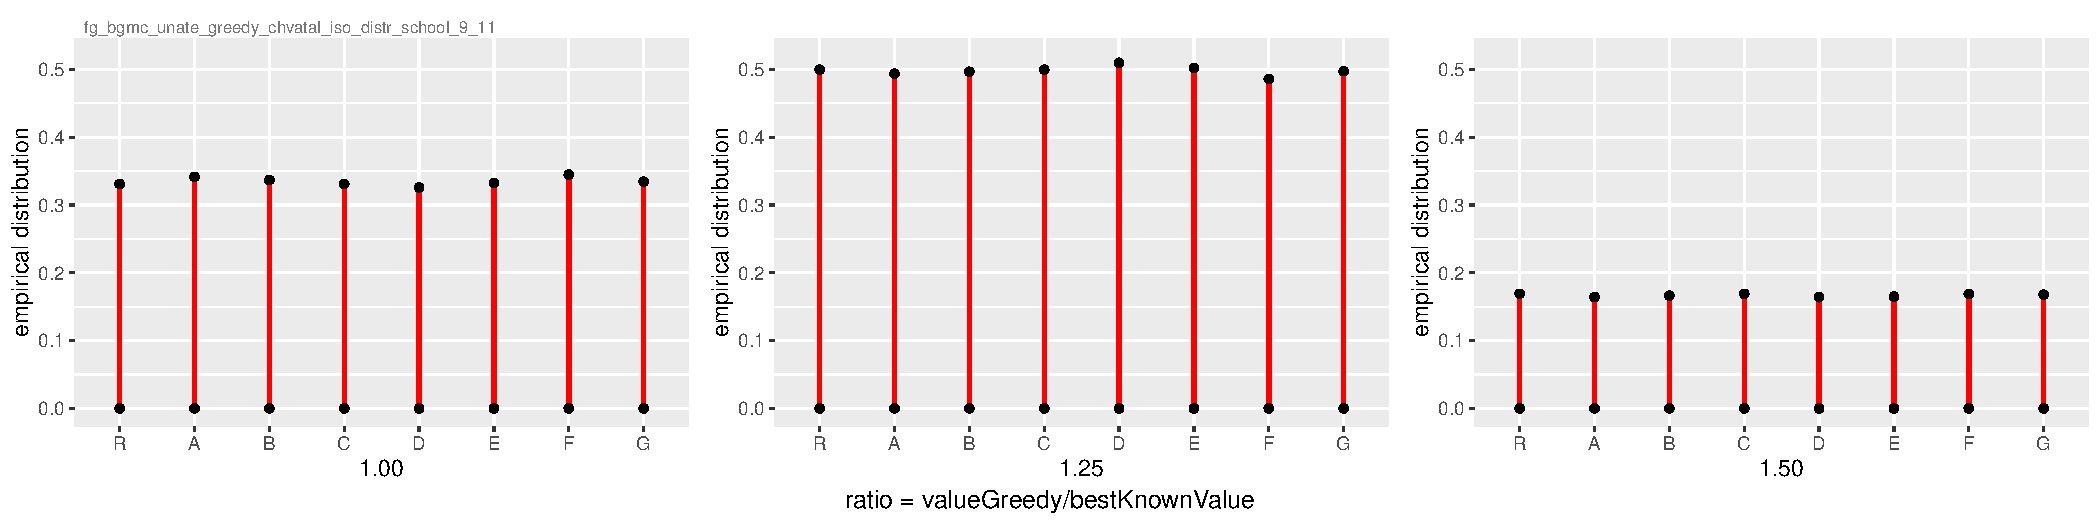
\includegraphics[width=0.90\textwidth]{_Figures/fg_bgmc_unate_greedy_chvatal_stoc_distr_school_9_11}
\\[2ex]
{\sf (ab)}\\
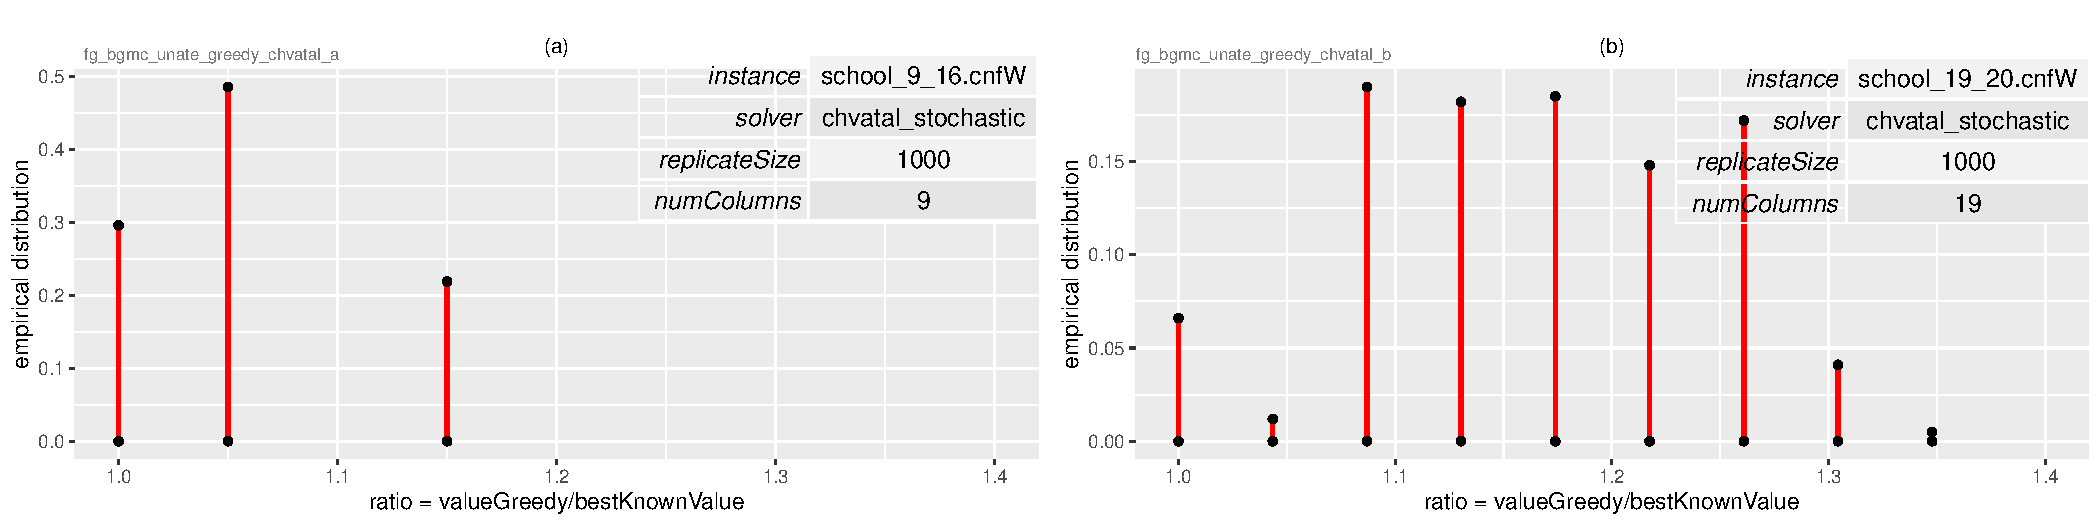
\includegraphics[width=0.90\textwidth]{_Figures/fg_bgmc_unate_greedy_chvatal_stoc_distr_ab}
\\[2ex]
{\sf (cd)}\\
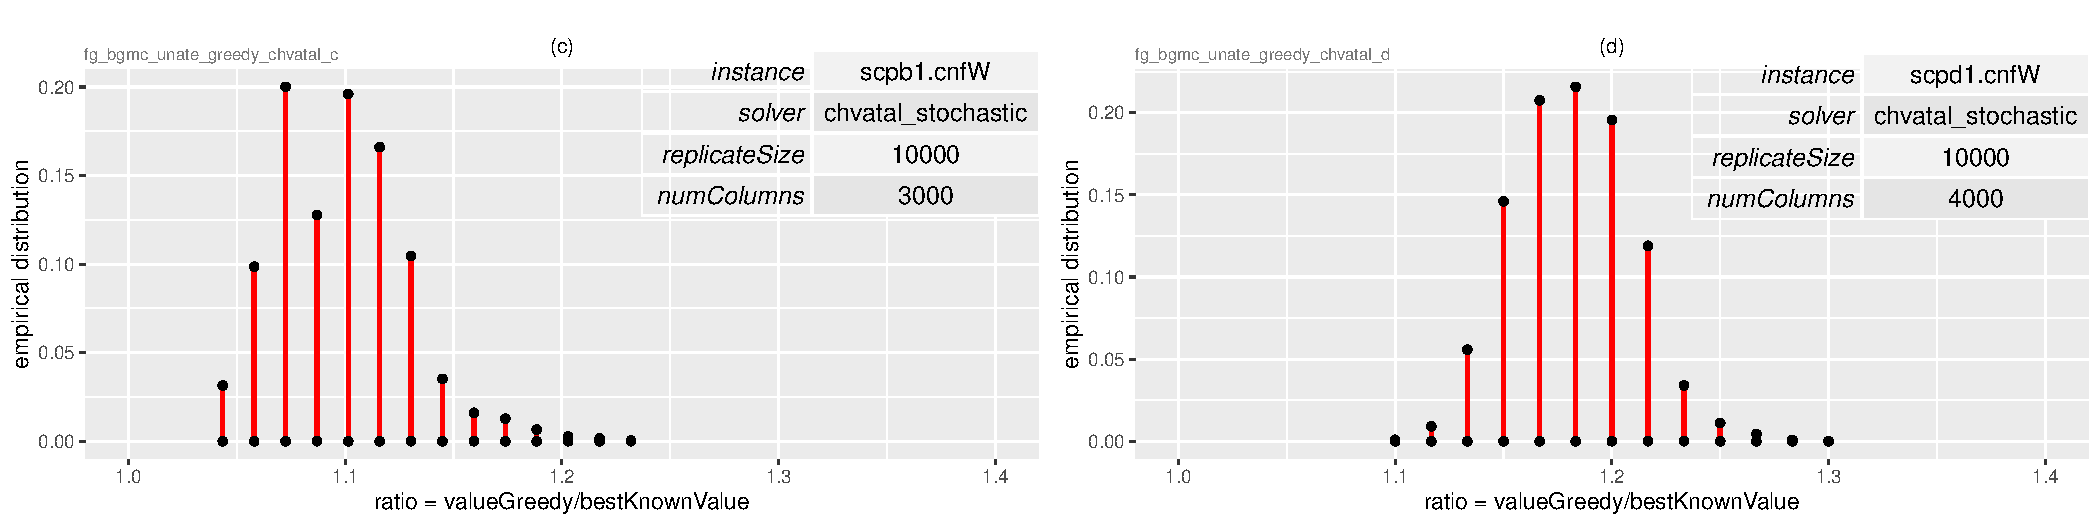
\includegraphics[width=0.90\textwidth]{_Figures/fg_bgmc_unate_greedy_chvatal_stoc_distr_cd}

\caption{
Reference parameters for each instance in this figure
are listed in Table~\ref{tb_bgmc_data}.
The top segment {\sf (school\_9\_11.cnfU)}
depicts  the empirical distribution of ratios \{1.0, 1.25, 1.5\}
for the 8 isomorph classes of size 10,000 each, induced by
the instance {\tt school\_9\_11.cnfU}. %
The middle segment {\sf (ab)}
depicts  distribution of ratios  
for two isomorph classes, each of size 1,000.
%
The bottom segment {\sf (cd)}
depicts  distribution of ratios the 
for two isomorph classes, each of size 10,000.
%
For additional details, see the article.
\vspace*{-3ex}
}
\label{fg_bgmc_unate_greedy_chvatal_stoc_distr}
\end{figure*}
